%%%%%%%%%%%%%%%%%%%%%%%%%%%%%%%%%%%%%%%%%%%%%%%%%%%%%%%%%%%%%%%%%%
%%  ~ Trabajo de Fin de Grado - Universidad de Vigo (ESEI) ~    %%
%% Autor: Diego Enrique Fontán Lorenzo                          %%
%% Tutor: Miguel Ramón Díaz-Cacho Medina                        %%
%% Convocatoria: Julio 2020/21                                  %%
%% Título: Framework de automatización de auditorías Red Team   %%
%%%%%%%%%%%%%%%%%%%%%%%%%%%%%%%%%%%%%%%%%%%%%%%%%%%%%%%%%%%%%%%%%%

%%%%%%%%%%%%%%%%%%%%%%%%%%%%%
%% OWASP
%%%%%%%%%%%%%%%%%%%%%%%%%%%%%

\chapter{OWASP -- Web Security Testing Guide} \label{anx:owasp}

En este anexo, se resumen algunas de las categorías habituales durante un \textit{pentesting} según la metodología \textit{OWASP}. En concreto, se hace referencia a la \textit{Web Security Testing Guide v4.2}. El documento original completo se puede encontrar en la siguiente dirección web: \url{https://owasp.org/www-project-web-security-testing-guide/v42/}.

\section{Contextualización} \label{sec:owaspdef}

\begin{quotation}
    \textit{``El Proyecto de Pruebas OWASP ha estado en desarrollo durante muchos años. El objetivo del proyecto es ayudar a la gente a entender el qué, el por qué, el cuándo, el dónde y el cómo de las pruebas de las aplicaciones web. El proyecto ha proporcionado un marco de pruebas completo, no sólo una simple lista de comprobación o una prescripción de cuestiones que deben abordarse. Los lectores pueden utilizar este marco como plantilla para construir sus propios programas de pruebas o para calificar los procesos de otras personas. La Guía de Pruebas describe con detalle tanto el marco general de pruebas como las técnicas necesarias para ponerlo en práctica.''} -- \textit{OWASP}
\end{quotation}

Hay que entender que las pruebas de seguridad nunca serán una ciencia exacta. No es posible llegar a definir una lista concreta con todos los posibles problemas que deben intentar solucionarse.\sn

El objetivo de la \textit{OWASP WSTG} es intentar recopilar el mayor número de pruebas, explicar las técnicas necesarias y mantener la guía actualizada. El método de pruebas de seguridad de aplicaciones web de \textbf{\textit{OWASP} se basa en el enfoque de caja negra}, es decir, el auditor no sabe nada o tiene muy poca información sobre la aplicación que va a probar.

\section{Categorías} \label{sec:owaspcat}

Las pruebas contenidas en la guía se agrupan por escenarios. Cada escenario tiene un identificador único, en el formato \textbf{WSTG-\textit{categoría}-\textit{control}}. La categoría es  una cadena de 4 caracteres en mayúsculas que identifica el tipo de prueba o debilidad, y el control es un número del 01 al 99. Por ejemplo: \textit{WSTG-INFO-03} es la tercera prueba de la categoría \textit{Recopilación de Información}.\n

La versión 4.2, usada como referencia durante el proyecto, consta de un total de noventa y siete controles, algunos de ellos con múltiples pruebas. Estos controles están agrupados dentro de doce categorías diferentes.\sn

La aplicación presentada como resultado del Trabajo de Fin de Grado descrito en este documento ofrece algunos \textit{ingredientes} ya definidos con los que poder realizar parte de los controles.\sn

Las pruebas cubiertas mediante estos nodos son los siguientes \tab{owaspingredients}.\sn

\begin{table}[H]
    \centering
    \begin{tabularx}{\textwidth}{| l | X |}
        \hline
        \multicolumn{2}{c}{ \textbf{Ingredientes de la categoría \textit{OWASP}} } \\ \hline
        \textbf{Identificador} & \textbf{Descripción} \\ \hline
        WSTG-INFO-01 & Reconocimiento con motores de búsqueda \\ \hline
        WSTG-INFO-02 (1) & \textit{Fingerprint} del servidor web \\ \hline
        WSTG-INFO-03 & Revisión de los archivos de \textit{metainformación} \\ \hline
        WSTG-INFO-04 (1) & Enumeración de aplicaciones web en diferentes \textit{URLs} \\ \hline
        WSTG-INFO-04 (2) & Enumeración de aplicaciones web en diferentes \textit{puertos} \\ \hline
        WSTG-INFO-04 (3) & Enumeración de aplicaciones web usando \textit{hosts} virtuales \\ \hline
        WSTG-INFO-05 & Revisión del contenido de la página web \\ \hline
    \end{tabularx}
    \caption{Ingredientes de la categoría \textit{OWASP}}
    \label{tab:owaspingredients}
\end{table}

Un ejemplo del uso de estos nodos mediante la aplicación es el mostrado en la figura \fig{owaspexample}.\sn

\begin{figure}[H]
    \centering
    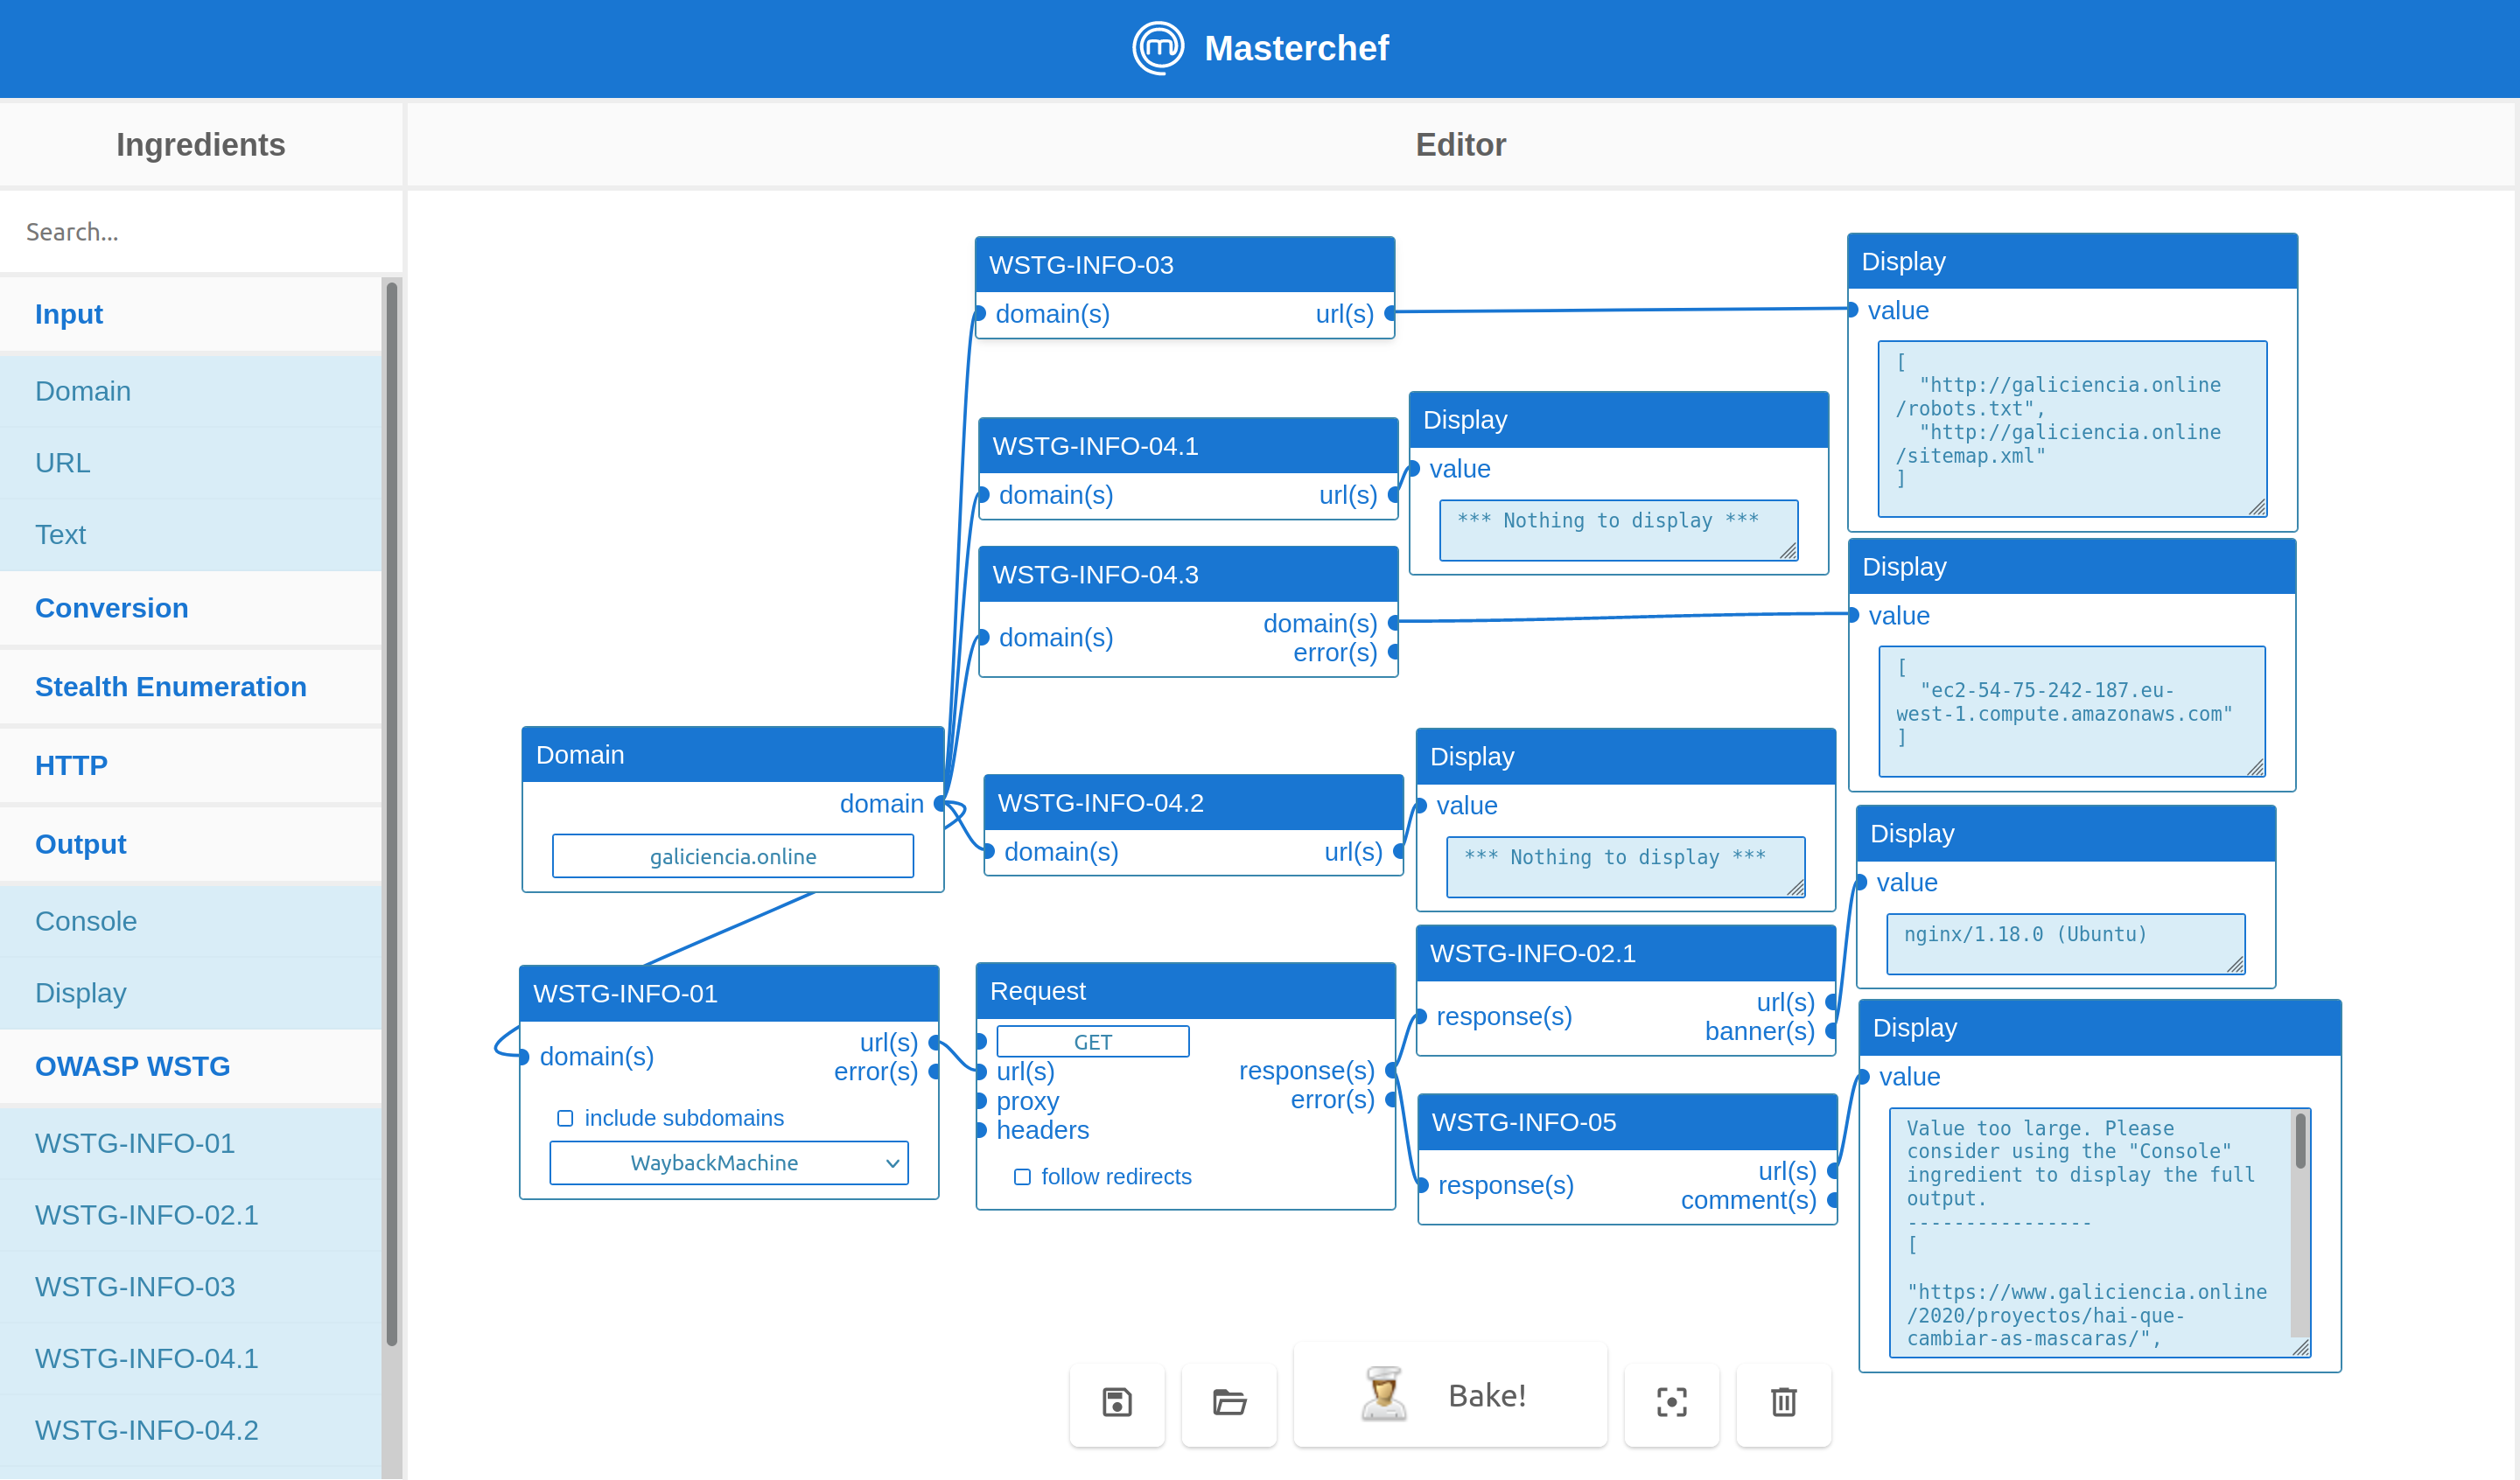
\includegraphics[width=15cm]{img/tables/34_Recipe-WSTG.png}
    \caption{Controles \textit{INFO} de \textit{OWASP WSGT}.}
    \label{fig:owaspexample}
\end{figure}